\subsection{Credit Analysis}

\begin{definition} \hlt{Credit Risk}\\
Risk associated with losses to fixed income investors, due to failure of borrower to make payment of interest or principal. When borrower fails to service their debt, they are in default.
\end{definition}

\subsection{Fundamentals of Credit Analysis}

\begin{figure}[H]
\centering
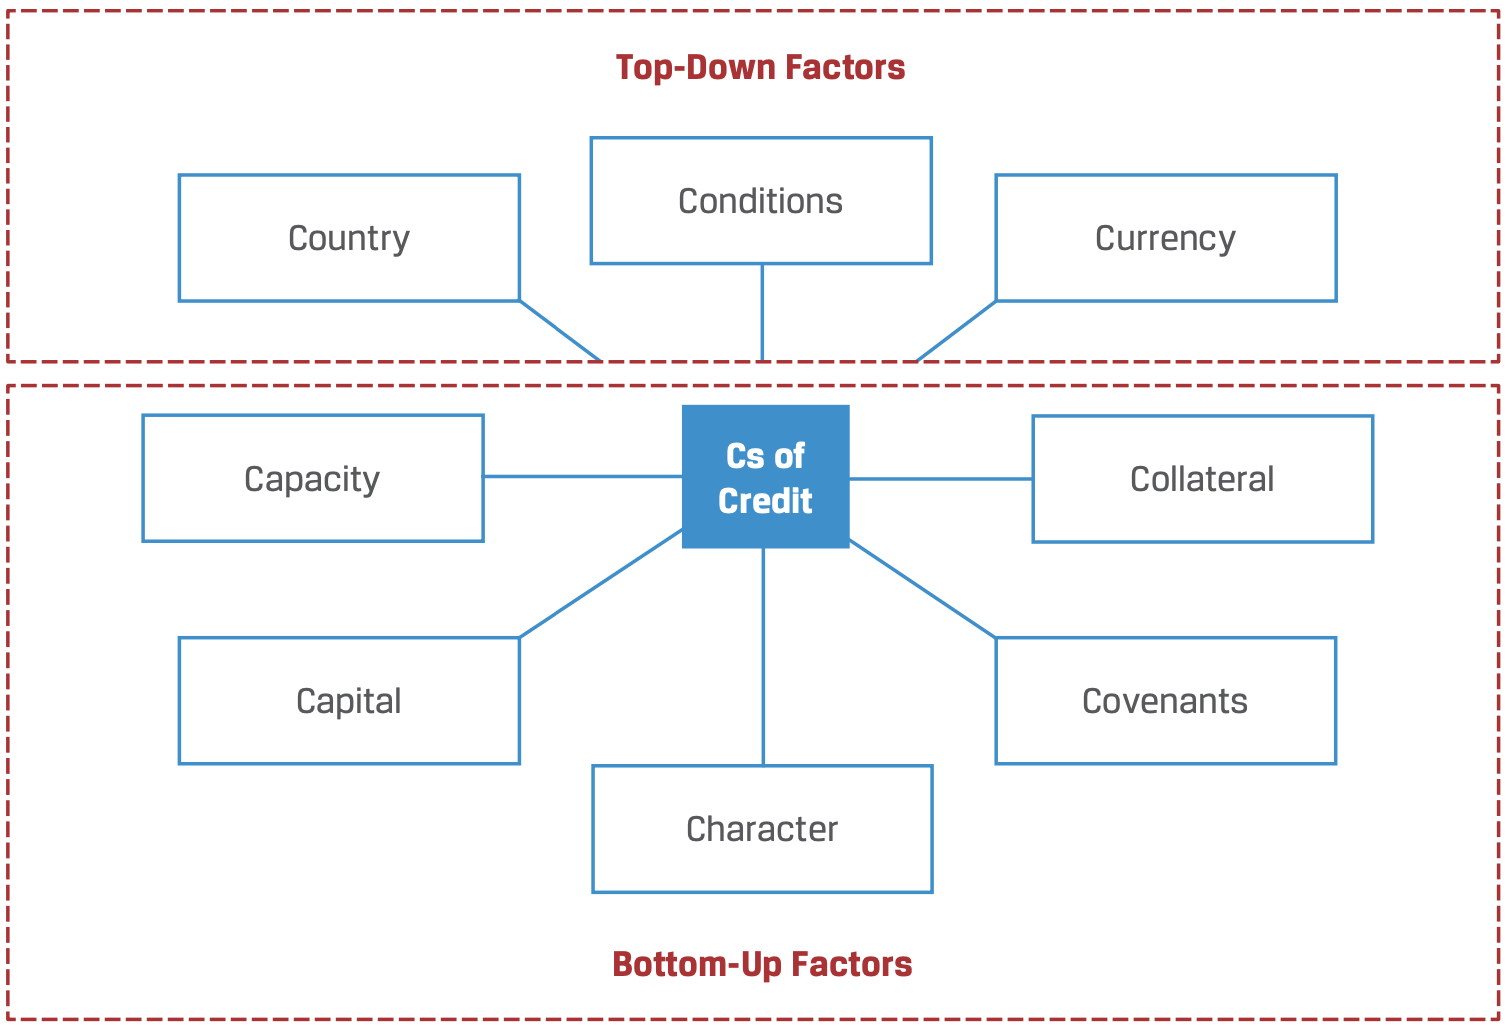
\includegraphics[scale=0.35]{/fi/csofcredit}
\caption{The Cs of Credit Analysis}
\end{figure}

\begin{remark} \hlt{Bottom-Up Credit Analysis Factors}
\begin{enumerate}[label=\roman*.]
\setlength{\itemsep}{0pt}
\item Capacity: measures borrower's ability to make debt payments on time
\item Capital: other resources available to borrower that reduce reliance on debt
\item Collateral: quality and value of assets supporting issuer's indebtedness
\item Covenants: legal terms and conditions the borrowers and lenders agree to as part of bond issue
\item Character: quality of management and willingness of repay indebtedness
\end{enumerate}
\end{remark}

\begin{remark} \hlt{Top-Down Credit Analysis Factors}
\begin{enumerate}[label=\roman*.]
\setlength{\itemsep}{0pt}
\item Conditions: general economic, competitive, and business environment faced by all borrowers that may affect their ability to service or refinance debt
\item Country: geopolitical environment, legal and political system faced by all issuers in a jurisdiction that may affect debt payment
\item Currency: affects issuers whose cash flows are affected by exchange rate changes or who borrow in a currency outside of their jurisdiction, such as sovereign issuers with foreign currency debt.
\end{enumerate}
\end{remark}

\begin{flushleft}
Borrower Types, Sources of Repayment, Sources of Credit Risk
\begin{tabularx}{\textwidth}{p{6.5em}|p{11em}|p{11em}|X}
\hline
\rowcolor{gray!30}
Borrower Type & Primary CF Source & Secondary CF Source & Credit Risk Source \\
\hline
Corporate & 
\xxx Business Operations
\xxx Investment, financing activities
&
\xxx Asset sales
\xxx Divestitures
\xxx Additional debt issuance
\xxx Equity issuance
&
\xxx Economic contraction
\xxx Strategic shifts in business and market environment
\xxx Increase competition
\xxx Reduced pricing power
\xxx Shrinking operating margin, increased losses
\xxx Excessive debt service needs \\
\hline
Soverigen or Public Entity & 
\xxx Taxes (income, sales, VAT, capital gains, wealth-based)
\xxx Tariffs, fees, other government revenue
&
\xxx Newly issued debt
\xxx Sale of public assets, privatisation
&
\xxx Economic contraction
\xxx Political uncertainty
\xxx Excessive debt service needs
\xxx Expansionary economic policies
\xxx Budget deficits
\xxx Tax cuts
\xxx Limited ability to collect taxes \\
\hline
\end{tabularx}
\end{flushleft}

\begin{figure}[H]
\centering
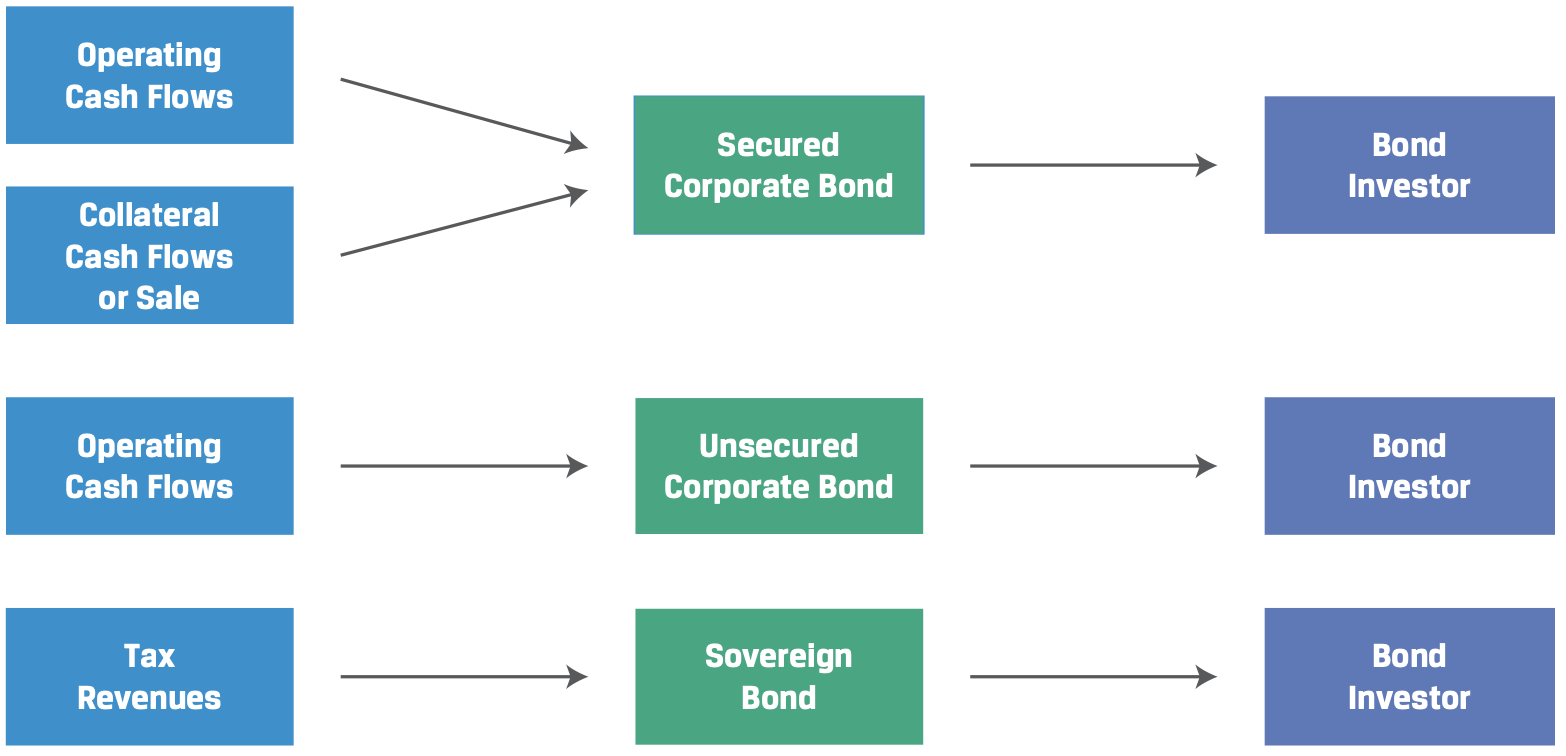
\includegraphics[scale=0.35]{/fi/sovcorpsourceofpayment}
\caption{Sovereign and Corporate Bond Sources of Repayment}
\end{figure}

\begin{remark} \hlt{Illiquid vs Insolvent}\\
Illiquid issuer is an issuer unable to raise cash to service debt.\\
Insolvent issuer has assets falling below the value of its debt.\\
An illiquid issuer may not necessarily be insolvent, but could still default.
\end{remark}

\begin{remark} \hlt{Bond Identure Clauses}
\begin{enumerate}[label=\roman*.]
\setlength{\itemsep}{0pt}
\item Cross-Default Clause: a default on one bond issuer causes a default on all issues
\item Pari Passu Clause: all bonds of certain type rank equally in the default process
\end{enumerate}
If both provisions exist on unsecured debt, a default on one issuer implies all holders of unsecured claims have access to general assets of the issuer to satisfy their obligations.\\
If both provisions exist on secured debt, default on any obligation of the issuer will grant access to general assets of the company and to assets pledged as collateral for the debt.\\
If value of pledged assets fall below amount of pari passu secured debt, secured bond investor have credit losses.
\end{remark}

\begin{remark} \hlt{Components of Credit Risk}
\begin{enumerate}[label=\roman*.]
\setlength{\itemsep}{0pt}
\item Probability of Default (POD): likelihood that issuer fails to make full and timely payments of principal and interest. Measure is typically annualised.
\item Loss Given Default (LGD): investor's loss conditional on issuer event of default. Combines severity of loss under fault scenario with amount of investor's claim at time of default.
\item Recovery Rate (RR): percentage of outstanding debt claim recovered when issuer defaults.
\item Loss Severity ($1 - \text{RR}$): unrecovered portion of the claim
\item Expected Exposure (EE) or Exposure at Default (EAD): amount an investor may expect to lose in case of default, equal to loan or bond face value plus accrued interest, less current market value of collateral.
\end{enumerate}
\begin{align}
\text{EL} &= \text{POD} \times \text{LGD} \nonumber \\
\text{LGD} &= \text{EE} \times (1 - \text{RR}) \nonumber
\end{align}
Using annualised EE as estimate of annualised credit spread over risk-free benchmark for credit risk,
\begin{equation}
\text{Credit Spread} \approx \text{POD} \times \text{LGD} \nonumber
\end{equation}
If actual credit spread of issue is higher than this estimated credit spread, investor is more than fairly compensated for the credit risk of the investment. 
\end{remark}

\begin{figure}[H]
\centering
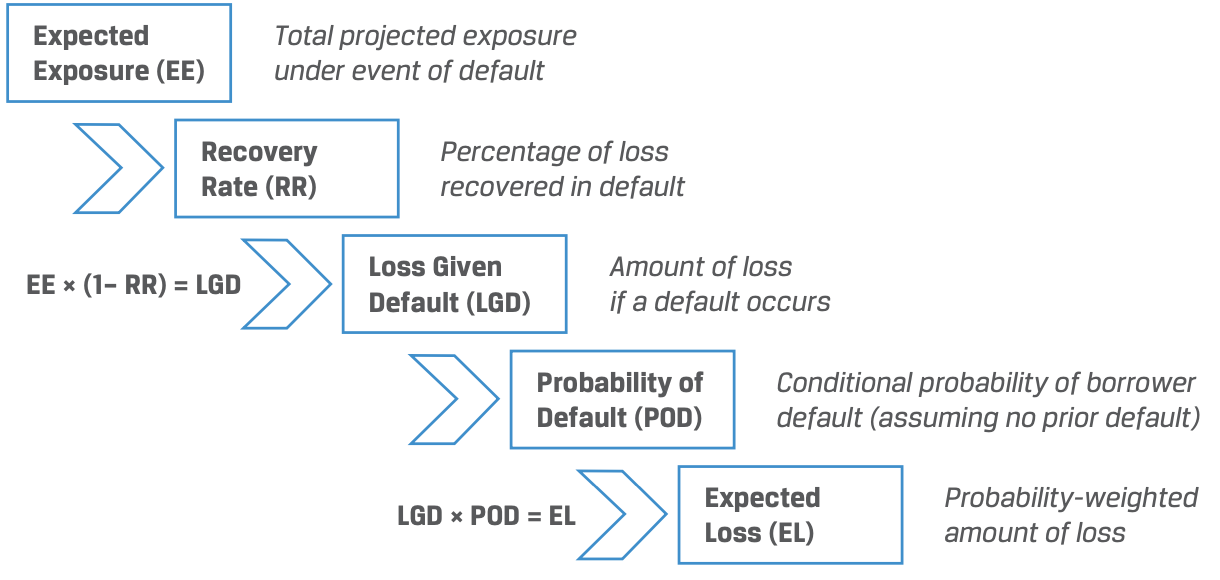
\includegraphics[scale=0.4]{/fi/creditriskcomp}
\caption{Components of Credit Risk}
\end{figure}

\begin{remark} \hlt{Drivers of Probability of Default}
\begin{enumerate}[label=\roman*.]
\setlength{\itemsep}{0pt}
\item Profitability: stable, predictable cash flows and profits. Higher is better.
\item Coverage: sufficient cash flows/profits to make debt payments. Higher is better.
\item Leverage: relative reliance on debt financing. Lower is better.
\end{enumerate}
\end{remark}

\begin{figure}[H]
\centering
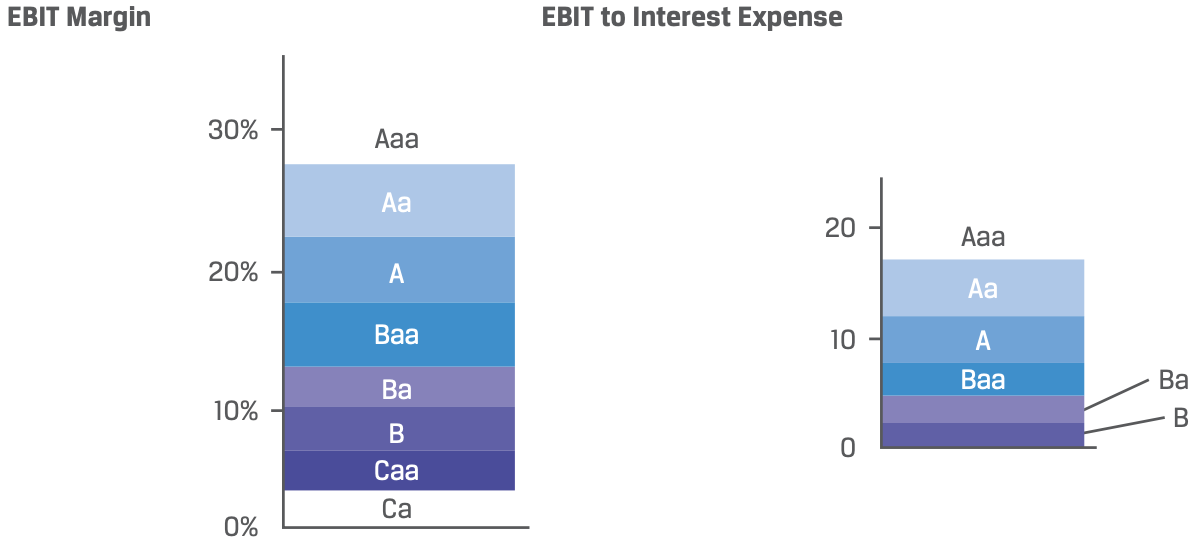
\includegraphics[scale=0.38]{/fi/keyfinratiocredit1}
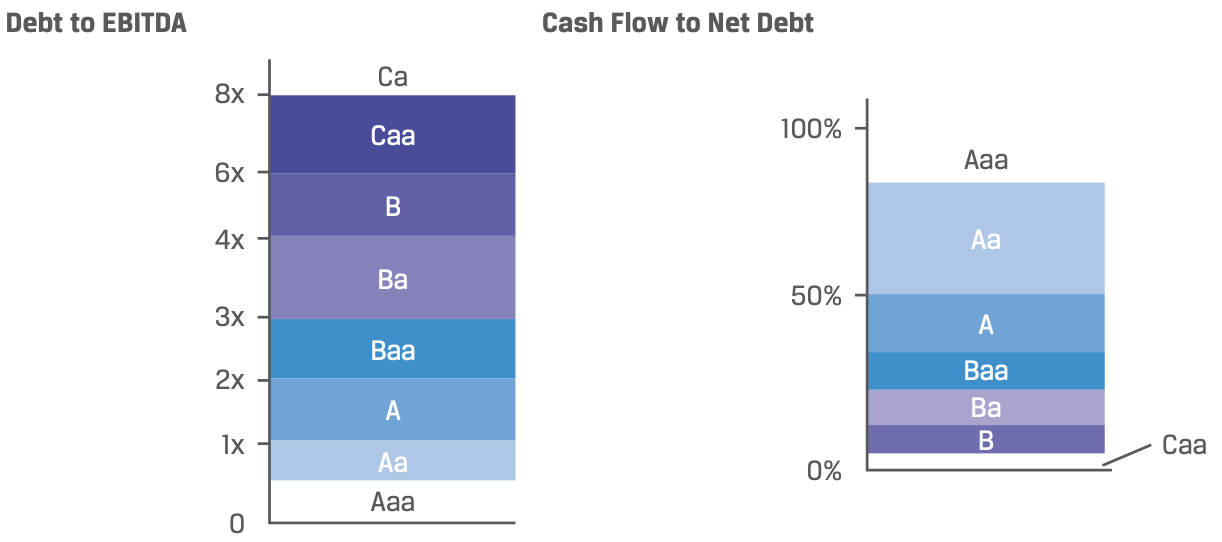
\includegraphics[scale=0.38]{/fi/keyfinratiocredit2}
\caption{Key financial ratios for corporate credit risk and ratings}
\end{figure}

\begin{remark} \hlt{Drivers of Loss Given Default}\\
A function of nature and seniority of creditor's claim in a default scenario.\\
More senior, secured debt will have lower losses given default than junior, unsecured debt.\\
High-yield issuer may issue secured debt with secondary source of repayment in event of default. Hence high-yield debt can have lower loss given default than unsecured bonds of investment grade issuer.\\
Greatest risk in unsecured investment grade debt is an increase in probability of default due to deterioration of issuer's financial situation.
\end{remark}

\begin{definition} \hlt{Hazard Rate (HR)}\\
Conditional probability of default given that default has previously not occured.
\end{definition}

\begin{definition} \hlt{Probability of Survival (POS)}\\
Assuming a constant hazard rate, at time $t$, 
\begin{align}
\text{POS}_t &= 1 - \text{Cumulative POD} \nonumber \\
&= (1-\text{HR})^t \nonumber \\
\text{POD}_t &= \text{HR} \times \text{POS}_{t-1} \nonumber
\end{align}
Note that POS decreases over time, and POD depends on POS from prior period.\\
In first year, POD $=$ HR, as PS $=1$ at inception. In subsequent periods, PD $<$ HR.
\end{definition}

\begin{definition} \hlt{Credit Valuation Adjustment (CVA)}\\
Sum of present value of expected loss for each period. CVA is monetary value of credit risk in present value terms; it is difference in value of risk-free bond and identical risky bond.
\begin{equation}
\text{CVA} = \text{Price of Risk-Free Bond} - \text{Price of Risky Bond} = \text{Sum of PV of Expected Loss}\nonumber
\end{equation}
\end{definition}

\begin{remark} \hlt{Risk Neutral Probability of Default}\\
Probability of default implied on current market price. Solve for POD below:
\begin{equation}
\text{Market Price of Bond} = \frac{\text{EE} \times (1-\text{POD}) + (1- \text{LGD})\times \text{POD}}{1 + \text{Benchmark Rate}} \nonumber
\end{equation}
The implied RR may also be derived from the equation, given POD.\\
If POD assumed is greater than the risk-neutral POD, then implied RR will be higher.\\
Given the market price and credit spread, risk neutral POD and RR are positive correlated.\\
Note that in the model, POD an RR are both estimates.
\end{remark}

\begin{remark} \hlt{ESG Considerations for Credit Risk}\\
Estimated POD and LGD to account for ESG-related risk exposure.\\
Climate and green bonds are issued with proceeds earmarked for environmental purposes, and may come with tax incentives to enhance attractiveness to investors.\\
Catastrophe and pandemic bonds resemble an insurance product, offering high interest payments in return for takin on risk of losing capital should a pandemic occur.
\end{remark}

\subsubsection{Credit Scores and Ratings}

\begin{remark} \hlt{Uses of Credit Ratings}
\begin{enumerate}[label=\roman*.]
\setlength{\itemsep}{0pt}
\item Comparing credit risk of issuers across industries and bond types, assessing changing credit conditions
\item Assessing credit migration risk (risk that credit rating downgrade will decrease value of bonds and potentially trigger other contractual clauses)
\item Meeting regulatory, statutory, or contractual requiremeents
\end{enumerate}
\end{remark}

\begin{flushleft}
Long-Term Rating Matrix, Investment Grade vs Non-Investment Grade
\begin{tabularx}{\textwidth}{p{9em}|p{8em}|X|X|X}
\hline
\rowcolor{gray!30}
Grade & Detail & Moody's & S\&P & Fitch \\
\hline
Investment & High-Quality & Aaa & AAA & AAA \\
& & Aa1 & AA+ & AA+ \\
& & Aa2 & AA & AA \\
& & Aa3 & AA- & AA- \\
& Upper-Medium & A1 & A+ & A+ \\
& & A2 & A & A \\
& & A3 & A- & A- \\
& Low-Medium & Baa1 & BBB+ & BBB+ \\
& & Baa2 & BBB & BBB \\
& & Baa3 & BBB- & BBB- \\
\hline
Non-Investment & Low, Speculative & Ba1 & BB+ & BB+ \\
(Junk, High-Yield) & & Ba2 & BB & BB \\
& & Ba3 & BB- & BB- \\
& & B1 & B+ & B+ \\
& & B2 & B & B \\
& & B3 & B- & B- \\
& & Caa1 & CCC+ & \\
& & Caa2 & CCC & CCC \\
& & Caa3 & CCC- & \\
& & Ca & CC & CC \\
& & Ca & C & C \\
& Default & C & D & D \\
\hline
\end{tabularx}
\end{flushleft}
Rating agencies also provide an outlook (positive, negative, stable).\\
Higher rated bonds trade at lower spreads relative to benchmark rates.

\begin{remark} \hlt{Limitations of Credit Ratings from Agencies}
\begin{enumerate}[label=\roman*.]
\setlength{\itemsep}{0pt}
\item Credit ratings lag market pricing. Two bonds with same rating may trade at different yields as credit ratings focus on expected loss, but market pricing for distressed debt focuses more on default timing and expected recoveries.
\item Risks such as litigation, natural disasters, environmental risks, acquisitions and equity buybacks using debt are not easily predicted or captured in credit ratings. Agencies may take different views on likelihood of such events, leading to split ratings.
\item Mistakes may occur; corporate fraud may lead to companies with high credit ratings suddenly defaulting.
\end{enumerate}
\end{remark}

\begin{remark} \hlt{FICO Score Factors}
\begin{enumerate}[label=\roman*.]
\setlength{\itemsep}{0pt}
\item $35\%$ Payment History: presence or lack of such information such as delinquency, bankruptcy, court judgments, repossessions, foreclosures
\item $30\%$ Debt Burden: credit card debt-to-limit ratios, $\#$ accounts with balances $>0$, total amount owed
\item $15\%$ Length of Credit History: average age of accounts on credit file, age of oldest account
\item $10\%$ Types of Credit Used: use of instalment payments, consumer finance, mortgages
\item $10\%$ Recent Searches for Credit: 'hard' credit inquiries when consumers apply for new loans
\end{enumerate}
\end{remark}

\begin{definition} \hlt{Credit Migration}\\
A change in rating reflects a change in bond's credit risk.\\
Change in price of the bond depends on modified duration of the bond, and change in spread resulting from change in credit risk as reflected by the credit migration.
\begin{equation}
\Delta \% \text{Price} = - \text{ModDur} \times (\Delta \text{Spread}) + \frac{1}{2} \text{Convexity}(\Delta \text{Spread})^2 \nonumber
\end{equation}
\end{definition}

\begin{definition} \hlt{Credit Spread Risk}\\
Risk that yield spreads widen due to deteriorating conditions, causing credit-risky bond prices to increase.\\
Credit spread risk arises from macroeconomic, issuer-specific, market related factors.
\end{definition}

\begin{remark} \hlt{Credit Spread Risk Macroeconomic Factors}
\end{remark}

